\chapter{Analog and digital signal transmission}
\begin{overview}
The different issues surrounding the implementation of the analog wiring system in the process control laboratory is discussed. This includes the layout design of a \eindex{junction box} for each individual \eindex{experimental setup} as well as the box used to house the A/D and D/A converter instrumentation. The different protocols with regard to the different cables used in the wiring of the analog system are also given.
\end{overview}
  
\section{Signal component installation}
An overview of the analog and digital signal transmission configuration as implemented in the control laboratory can be seen in figure~\ref{fig:wire:over}. 
\begin{figure}[htbp]
	\centering
	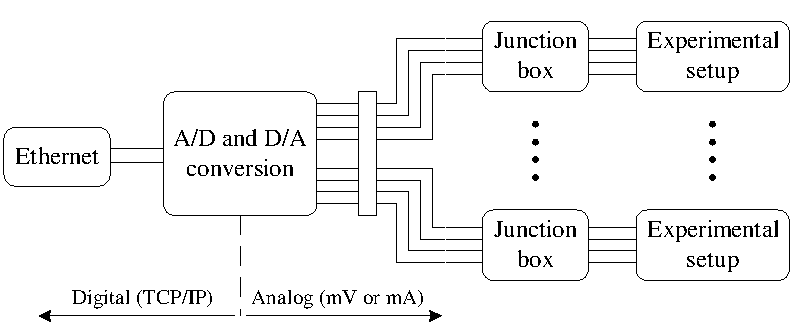
\includegraphics[width = 0.8\textwidth]{wiringover}
	\caption{Analog and digital implementation}
	\label{fig:wire:over}
\end{figure}

The analog to digital and digital to analog converters is used to transform the analog signals to a digital networking protocol called (TCP/IP) and \emph{vice versa}. All the transmission lines of the experimental setups is routed to a centralised case or box (referred to as the \eindex{Opto box}) where the A/D and D/A conversion instrumentation is situated. The box is used to protect the expensive instrumentation as well as the open connections from dust and spills and the implementation thereof can be seen in figure~\ref{fig:wire:obox}.
\begin{figure}[htbp]
	\centering
	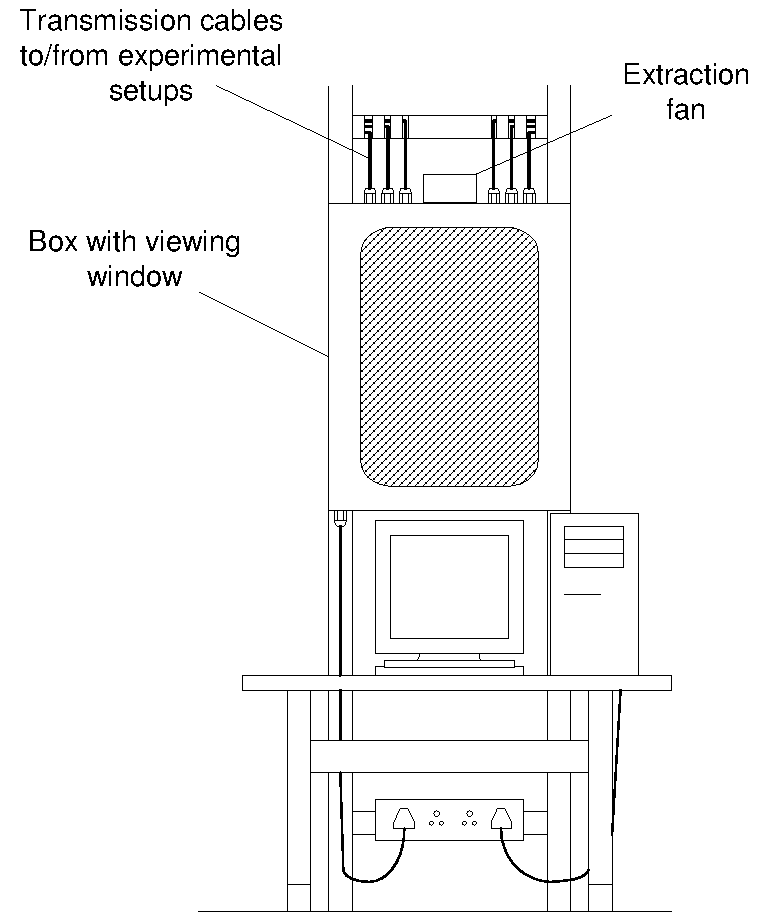
\includegraphics[width = 0.7\textwidth]{wireobox}
	\caption{Opto box installation}
	\label{fig:wire:obox}
\end{figure}

The \eindex{junction box} is inserted between the A/D and D/A converters and the instrumentation of the experimental setup and is used to:
\begin{itemize} 
	\item house the different power supplies needed for the instrumentation.
	\item create a physical connection point between the transmission lines in the trunking and that used to wire 				the experimental setup. 
	\item protect the instrumentation by inserting fuses in the transmission lines.
	\item create a save environment for the open connections and power supplies. 
\end{itemize}
The \eindex{junction box} is installed against the wall at each experimental setup together with the associated computer of the experimental setup. A graphical representation of the implementation of the \eindex{junction box} can be seen in figure~\ref{fig:wire:box}.
\begin{figure}[htbp]
	\centering
	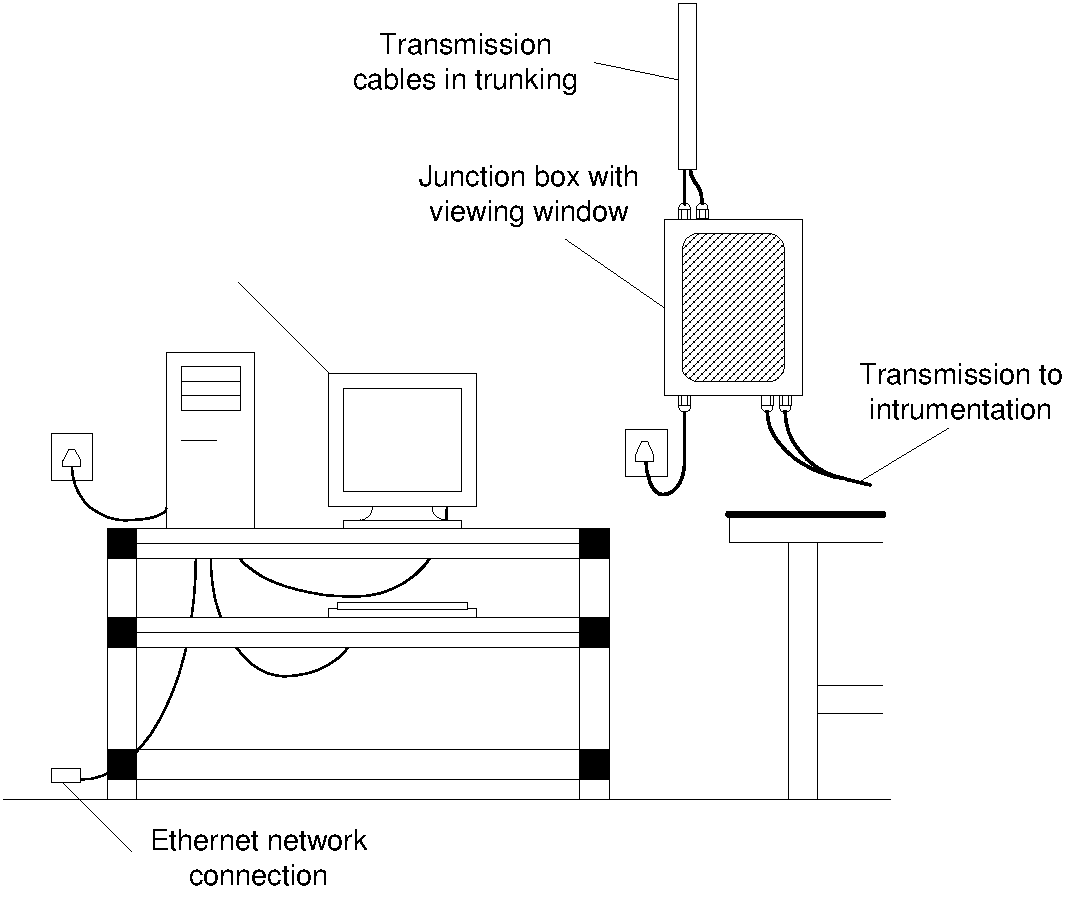
\includegraphics[width = \textwidth]{wirebox}
	\caption{Junction box installation}
	\label{fig:wire:box}
\end{figure}

The cables from the \eindex{Opto box} is situated in trunking (to keep the appearance of the process control laboratory neat) and enters the box at the top using cable glands to seal the box from dust and spills. The power cable and the cables that connects the instrumentation of the experimental setup to the junction box is separated to reduce noise contamination of the high voltage power cable on the measurement cables.

\section{Analog and digital input output instrumentation}    
The instrumentation used for the A/D and D/A conversion is the \eindex{SNAP ETHERNET I/O range} from OPTO22 and consist out of different individual components each with a specific function. A schematic of the interaction of the different components can be seen in figure~\ref{fig:wire:optoi}. 
\begin{figure}[htbp]
	\centering
	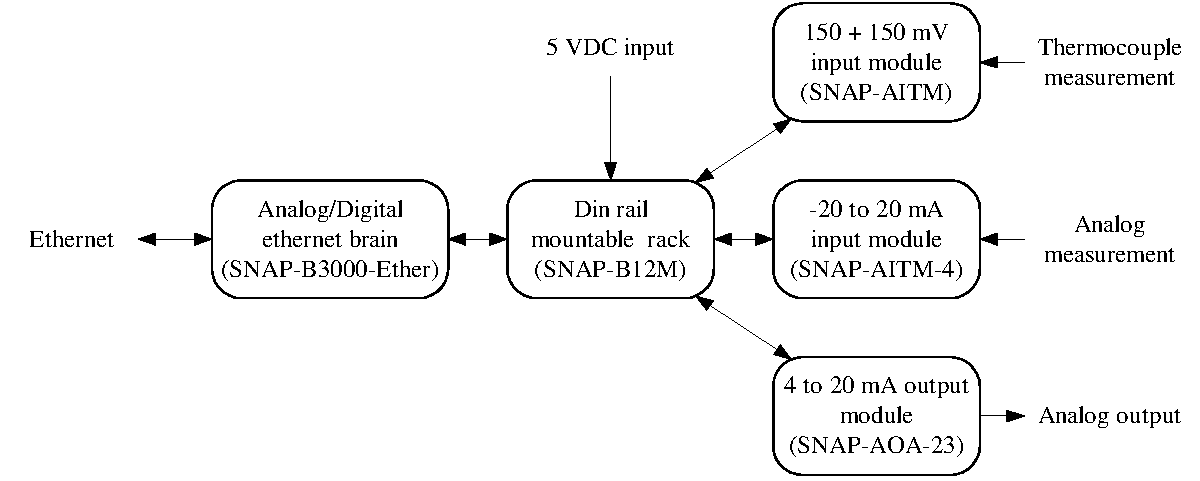
\includegraphics[width = \textwidth]{wireoptoi}
	\caption{Component specification of the SNAP I/O range}
	\label{fig:wire:optoi}
\end{figure}
Two different input modules are used for general process measurement (AITM--4) and thermocouple measurement (AIMA). One output module (AOA--23) is used for the manipulation of the actuators. The \eindex{AIMA} and \eindex{AOA--23} model has two channels while the \eindex{AITM--4} has four channels per module. The modules slot onto the \eindex{B12M rack} that is capable of housing a total of twelve modules. A breakdown of the different modules used can be seen in table~\ref{tab:wire:node} and shows that two racks are needed to house the twenty four modules
\begin{table}[htbp]
	\centering
	\caption{Module breakdown}
	\begin{tabular}{l c c}
	\toprule[1pt]
		Module name    &Channels&Modules \\
	\midrule[0.5pt] 
	  SNAP--AITM--4  &  18    &  5 \\ 
	  SNAP--AIMA     &  21		&  11\\
	  SNAP--AOA--23	 &  15    &  8 \\
	 \midrule[0.5pt]
	  Total          &  54    &  24\\
	 \bottomrule[1pt]
	\end{tabular}
	\label{tab:wire:node}
\end{table}

Every rack needs one \eindex{B3000 brain} and is used to convert the digital signal to the \eindex{TCP/IP} format, a protocol used to transfer data across the \eindex{ethernet}. The brain can be interfaced with:
\begin{description}
	\item [Modbus] which is a generic protocol devised for interfacing with third--party hardware and software. \index{Modbus} 
	\item [OPC] (object linking and embedding for control), a control protocol specifically devised for third--party software interfacing. The brain acts as an \eindex{OPC server} that can be interfaced with OPC and DDE clients.  \index{OPC} \index{DDE client} \index{OPC client}
	\item [ActiveX] (object linking and embedding for Windows) that was developed for third--party software interfacing \index{ActiveX}
	\item [HTML] that is a generic web based protocol used extensively as a communication medium on the \eindex{internet} \index{HTML} 
\end{description}

\section{Loop power}
The measuring equipment and actuators need electrical power to convert the physical properties of the process to an electrical signal that can be used for digital control and monitoring. The electricity is obtained either from the inputs used for the measurement output or as a different input supply. The use of the electrical power from the measurement signal is commonly referred to as \eindex{loop power}. 

A power supply must accordingly be used to power the signal transmission, but it is impractical to use one power supply for one measuring device. The power supply ($ES$) is therefore placed in parallel to the instruments ($XI$) requiring the power supply as can be seen in figure~\ref{fig:wire:ploop}. The A/D or D/A device ($OP$) is placed in series with the measuring instrument or actuator as it must measure or manipulate the signal. 
\begin{figure}[htbp]
	\centering
	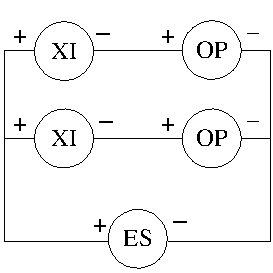
\includegraphics[width = 0.25\textwidth]{wireploop}
	\caption{Power supply implementation}
	\label{fig:wire:ploop}
\end{figure}

\section{Junction box layout}
The \eindex{junction box} is a powder painted mild steel case with a sealed hinged door with an IP55 rating (resistant to dust). A polycarbonate window was inserted into the door for illustrative purposes. A stainless steel base plate is inserted at the bottom of the box. Two C--rails are place vertically onto the base plate with bolts(see figure~\ref{fig:wire:jb}). 
\begin{figure}[p]
	\centering
	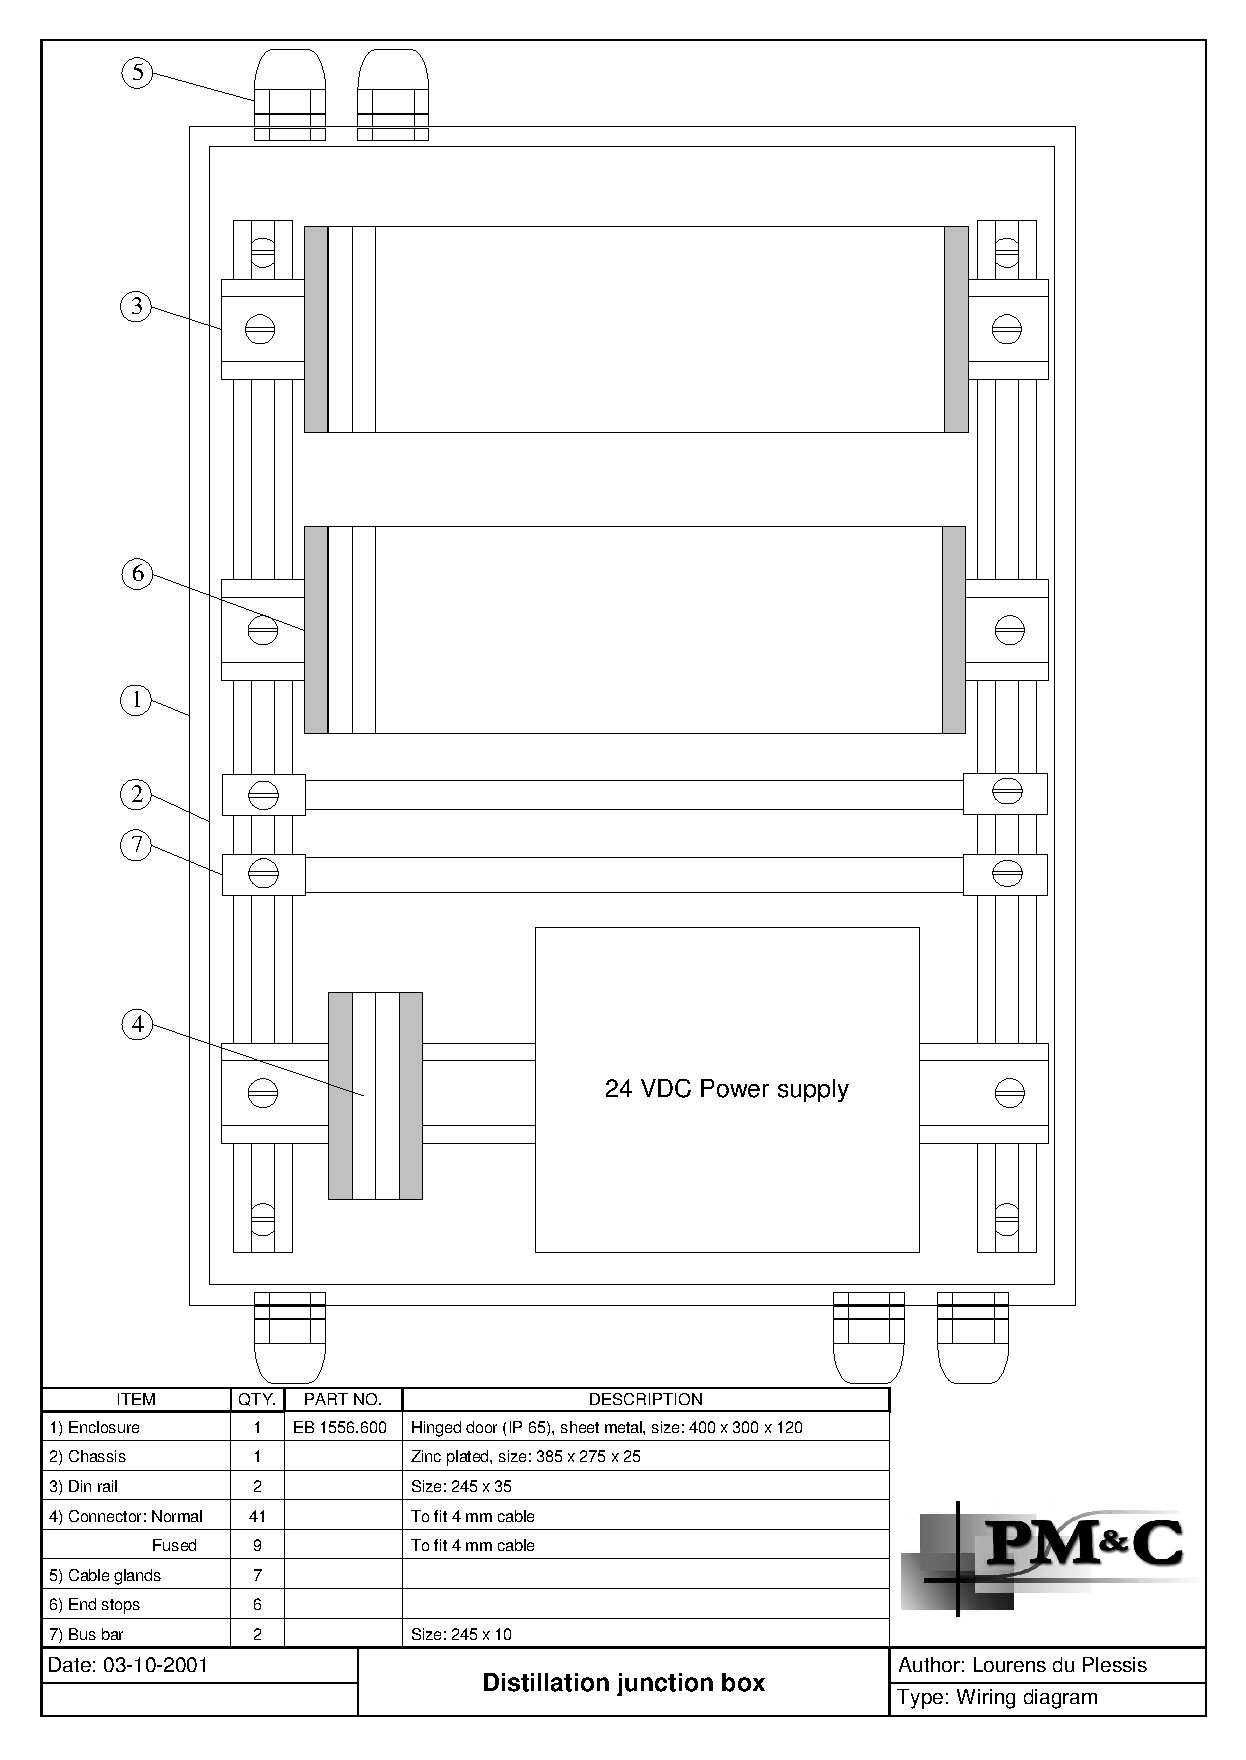
\includegraphics[width = \textwidth]{wirejb}
	\caption{Junction box layout}
	\label{fig:wire:jb}
\end{figure}

The \eindex{DIN rails} and \eindex{bus bars} are mounted onto the rails and tightened with bolts. The \emph{bus bars} and \emph{DIN rails} can therefore move freely once the bolts are loosened to give a larger degree of freedom to the box layout. The fused and normal \eindex{connectors} are specifically designed to ``clip'' onto the DIN rail and is used to connect two cables. The power supply is also placed onto the DIN rial and ensures the easy removal of the device as the base plate with all the other components need not be removed. The cables that enter the box at the top and bottom is sealed using \eindex{cable glands}. 

The \eindex{loop power} supplied by the 24V power supply is installed, in parallel with each  measuring or control loop, inside the \eindex{junction box} with the use of the \eindex{connectors} and the \eindex{bus bars}. The details can be seen in figure~\ref{fig:wire:loopp} and is based on the wiring diagram in figure~\ref{fig:wire:ploop}. 
\begin{figure}[htbp]
	\centering
	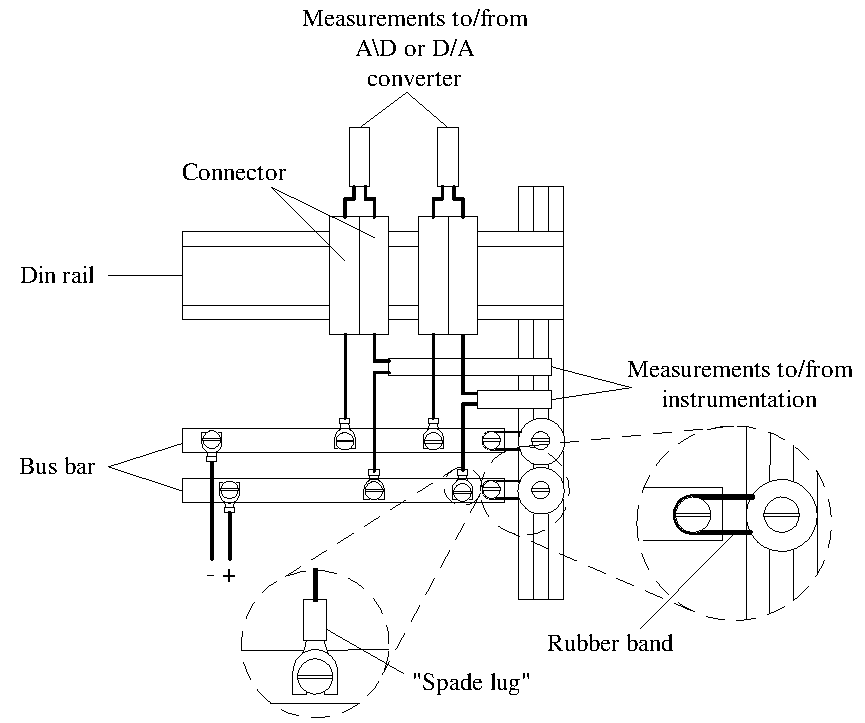
\includegraphics[width = 0.8\textwidth]{wireloopp}
	\caption{Loop power installation}
	\label{fig:wire:loopp}
\end{figure}
The \eindex{bus bar} is fixed to the C--rail by rubber bands to insulate the bar from the rest of the junction box. The cables can accordingly be fixed onto the \eindex{bus bar} with bolts and ``spade lugs''.
 
\section{Opto box layout}
The layout of the \eindex{Opto box} is based on the same principles as that of the \eindex{junction box}. The A/D and D/A instrumentation (OPTO22) are fitted to the DIN rail using custom clips and the power requirements of the instrumentation are supplied by two 5 VDC power supplies also fixed to the DIN rail.

A 220 VAC extraction fan is installed at the top of the box to remove the heat generated by the instrumentation. An air filter is installed at the bottom to act as the cool air inlet for the flow caused by the extraction fan.  
\begin{figure}[p]
	\centering
	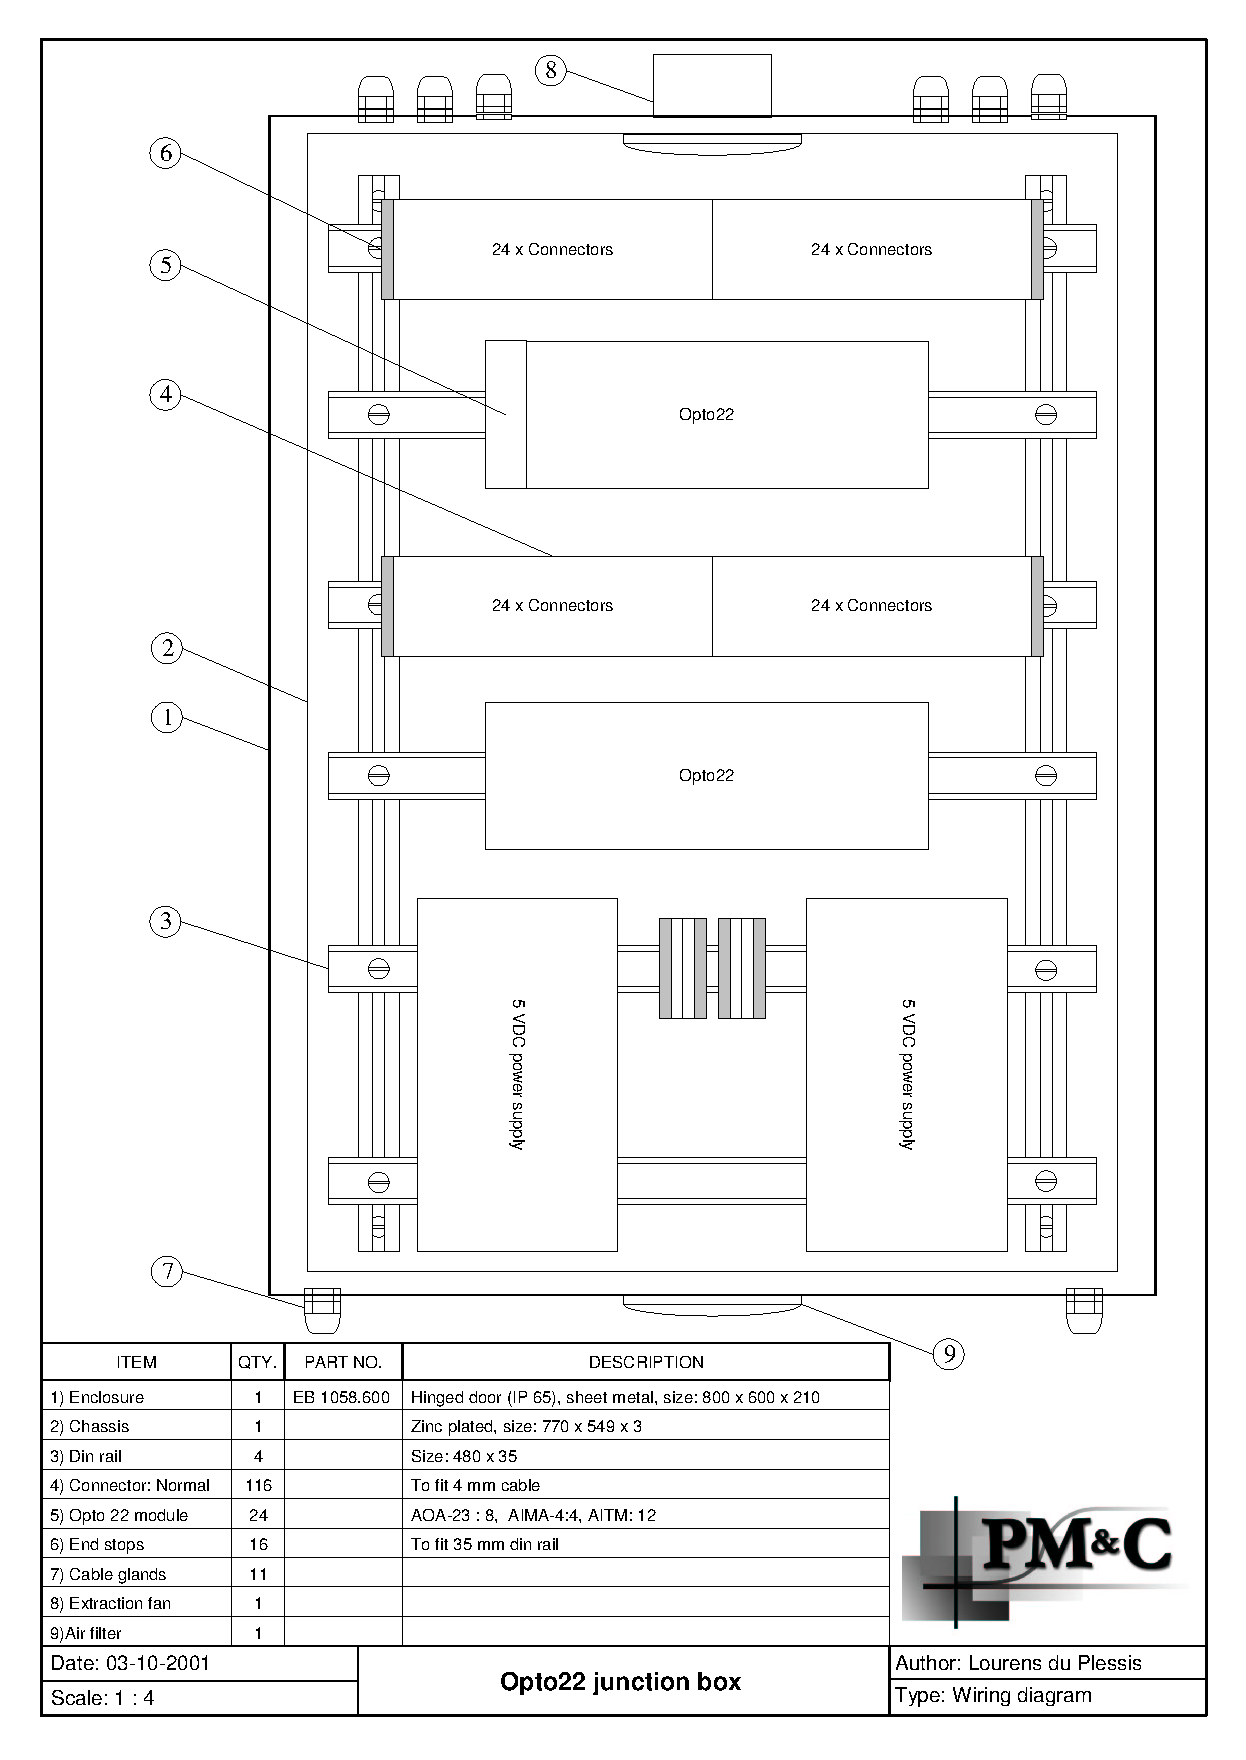
\includegraphics[width = \textwidth]{wireoptol}
	\caption{Opto box layout}
	\label{fig:wire:optol}
\end{figure}

\section{Cabling}
\subsection{Communication transmission}
The cable used for communication is \eindex{twisted pair shielded} cable with the shield placed between the outer and the inner insulation of the two individual conductors (see figure~\ref{fig:wire:comm}). This is to shield the signal in the conductors from external noise effects such as generators, heating coils, AC currents, etc. The outer insulation should be gray in colour and the two inner insulated conductors red and blue.
\begin{figure}[htbp]
	\centering
	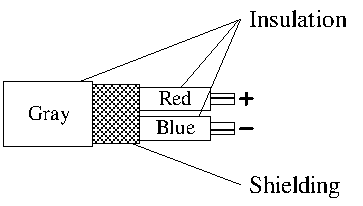
\includegraphics[width = 0.4\textwidth]{wirecomm}
	\caption{Cable used for communication}
	\label{fig:wire:comm}
\end{figure}

\subsection{Thermocouple measurement}
The cable used for the transmission of signal originating from thermocouples can be seen in figure~\ref{fig:wire:thermo}. The colour of the outer insulation is black while the inner insulation differs with the different type of thermocouple used. The colour scheme shown in figure~\ref{fig:wire:thermo} is that of a J--type thermocouple. The colour scheme for a K--type thermocouple is blue and yellow.
\begin{figure}[htbp]
	\centering
	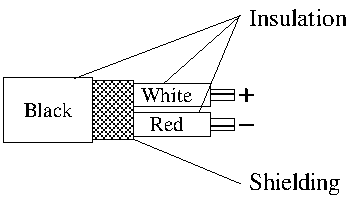
\includegraphics[width = 0.4\textwidth]{wirethermo}
	\caption{Cable used for thermocouple measurement}
	\label{fig:wire:thermo}
\end{figure}

\subsection{Power transmission}
Certain transmitters requires an extra power input. The cables used for this will therefore not be responsible for communication and must therefore be specified differently from the cable that is used for communication. The cable and colour scheme used for the purpose of power transmission for three  and two wire applications can be seen in figure~\ref{fig:wire:power} and figure~\ref{fig:wire:power2}. No shielding from electrical disturbances is needed as the cable is not used for communication. The voltages transmitted are also higher and are therefore not as susceptible to noise.
\begin{figure}[htbp]
  \centering
  \subfigure[Three wires]{
	  \hspace{3em}
  	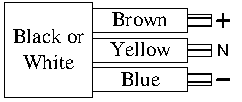
\includegraphics[width=0.3\textwidth]{wirepower}
  	\label{fig:wire:power}
	  \hspace{3em}
  }  
  \subfigure[Two wires]{
	  \hspace{3em}
  	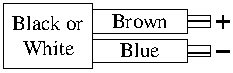
\includegraphics[width=0.3\textwidth]{wirepower2}
  	\label{fig:wire:power2}
	  \hspace{3em}
  }
 	\caption{Cable used for power transmission}
\end{figure}     

Power cables must be marked clearly with a tag stating the voltage and current type (i.e AC for alternating current or DC for direct current). This is necessary to ensure safe operation by reducing the risk of instrument damage and electrification. An example where a 220 VAC power line is marked can be seen in figure~\ref{fig:wire:mark}.
\begin{figure}[htbp]
	\centering
	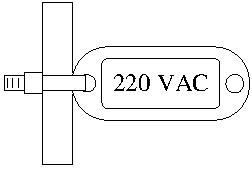
\includegraphics[width = 0.3\textwidth]{wiremark}
	\caption{Power cable marker}
	\label{fig:wire:mark}
\end{figure}

A ferrule, figure \ref{fig:digi:fer}, is placed over the exposed end points of the two conductors in the cables. This is to ensure a good (neat) connection of the cable in the connector; as the wire won't be able to bend because ferrule is rigid. 
\begin{figure}[htbp]
	\centering
	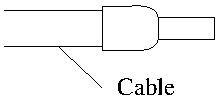
\includegraphics[width = 0.25\textwidth]{digifer}
	\caption{Ferrule placed on the end of the conductor}
	\label{fig:digi:fer}
\end{figure}    